\chapter*{Secondary Contributions}
\addcontentsline{toc}{chapter}{Secondary Contributions}
\label{Secondary_Contributions}

\textbf{PET FDG Improved Tumour Definition using Deep Learning}

Within the \gls{hybrid} schedule secondments, a 1-month secondment for Laura Dal Toso (LDT) from King's College London (KCL) was planned to take place at our lab. This secondment aimed in working on simulations for creating pairs of datasets, to be used for training Deep Learning (DL) methods used towards the improvement of PET images.

For applications of PET imaging in oncology, quantification and shape of tumours are regularly used by medical professionals for the characterisation and classification of disease. For the case of \gls{nsclc} imaging, and not only limited to that, these image characteristics are often degraded by image noise and partial volume effects.
In this work, a method for improving tumour shape definition and quantification was proposed, by use of Deep Learning (DL). As DL methods require a large number of training datasets, simulations were used to train the proposed DL method. 

The aim was to ultimately use the DL method for real \gls{nsclc} image data from an mMR PET/MR scanner (installed at KCL). Thus the implementation of the mMR geometry in the PET analytical simulator was needed, which was performed by me (ZC) with guidance from Dr Simon Stute. After the successful integration of the geometry for simulations and validation of reconstructions using CASToR, a large dataset of ground truth tumours (placed within the XCAT phantom) were simulated by LDT and provided for PET simulation. A total of 2210 cases were simulated and reconstructed, using a custom made pipeline by ZC on two computer clusters.
Details on the methodology used and results are provided in the attached draft paper, which will be submitted for publication.

\textbf{Data Driven Motion Correction for Brain PET Dynamic Imaging}

A 2-week secondment has been planned with \gls{hybrid} at the MUW in Vienna, with the aim of making use of dynamic reconstruction techniques developed during this PhD project to a cohort of epilepsy dynamic PET data. But this secondment was performed mostly by distance due to the pandemic and the time was spent towards the implementation and evaluation of motion estimation method for dynamic brain PET. 

The used datasets were acquired on an mMR PET/MR scanner, using MR sequences to track motion. But since access to PET/MR scanners is not always possible, there is need for accurate data-driven motion estimation techniques using PET only data. 

Towards this goal, a method was developed using ultra-short frame reconstruction 
and a Cycle Generative Adversarial Network (cGAN) to improve image quality for better motion estimation. 
For this project an raw data to CASToR datafile converter was developed by me in order to support conversion of dynamic data including all corrections. Using the converted data, dynamic reconstructions were performed in CASToR, using involuntary motion correction within the reconstruction, to result to motion free activity and parametric images. 

The development work and application of the cGAN has resulted in the attached publication by Shiyam Sundar \textit{et al.}~\cite{ShiyamSundar2020}. The work performed using CASToR has not been included in this publication, but it is considered for use in a future project on the topic of motion correction.

\cleardoublepage
\includepdf[pages=-]{SecondaryContributions/Formatted_Paper.pdf}
\cleardoublepage
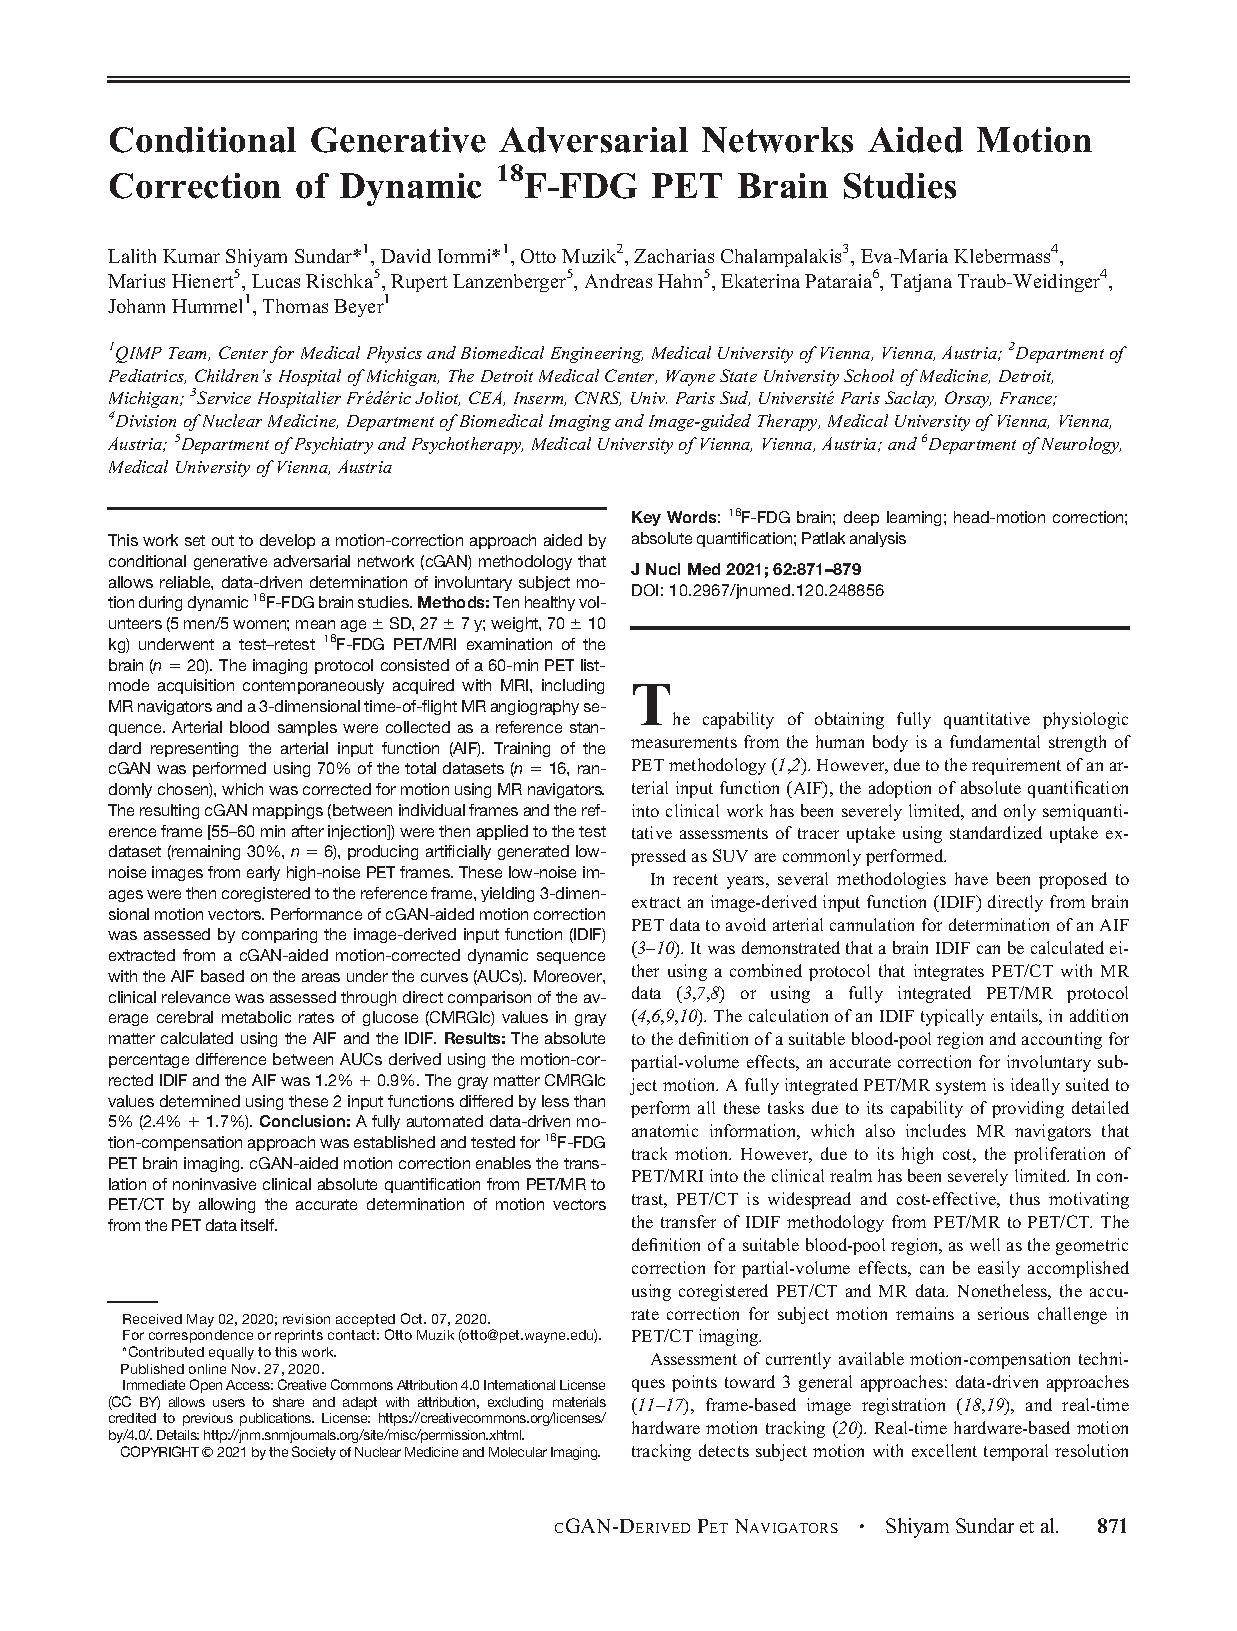
\includepdf[pages=-]{SecondaryContributions/871.full.pdf}